\chapter{Dispersión, dualidad y amplitud de Veneziano}

\lectureoverview{La dispersión reduce una colisión a datos invariantes que pueden compararse con los experimentos. Para cuatro partículas idénticas, esos datos pueden organizarse mediante las variables de Mandelstam \(s,t,u\), de las cuales solo dos son independientes. El intercambio ordinario de partículas sugiere entonces canales directo y cruzado separados. La amplitud de Veneziano cambió esa expectativa: una misma función contiene las descripciones de ambos canales. En la segunda mitad de la clase construiremos esa función a partir de dos cuerdas abiertas que se unen, evolucionan como una sola cadena oscilante y vuelven a separarse.}

\section{Qué debe predecir una teoría}

Las cuerdas fermiónicas resuelven dos problemas del modelo puramente bosónico: admiten estados fermiónicos y, tras la proyección adecuada, eliminan el taquión. Su dimensión crítica del espacio-tiempo es diez, en lugar de veintiséis. Por tanto, siguen existiendo dimensiones adicionales, pero dejaremos para más adelante su compactificación. El tema inmediato es la dispersión.
\editorialnote{La afirmación de que no hay taquiones se refiere al espectro consistente de supercuerdas después de la proyección requerida; añadir fermiones de hoja de mundo, por sí solo, no basta.}

La dispersión no es necesariamente lo más interesante que hacen las partículas. Es, sencillamente, la operación que un experimento puede repetir de forma controlada. Se envían partículas especificadas unas hacia otras, se registran las que salen de la colisión y se infiere la dinámica oculta en la región de interacción. Una teoría se vuelve cuantitativa cuando proporciona una amplitud compleja
\begin{equation}
  \mathcal A(\hbox{incoming data}\to\hbox{outgoing data}),
\end{equation}
cuyo módulo al cuadrado, junto con los factores habituales del espacio de fases, da la probabilidad de ese resultado.

\begin{figure}[H]
  \centering
  
\includegraphics[width=0.72\textwidth]{lecture_06_figure_01.png}
  \caption{Las partículas entrantes llegan a una región de interacción representada como una caja negra, y de ella salen partículas; el tiempo se representa en el eje horizontal.}
  \lectureframe{00:02:35}
  \label{fig:l06-black-box}
\end{figure}

Las partículas también llevan etiquetas de espín, carga y especie. Para exponer primero la cinemática, dejemos provisionalmente de lado todo salvo el momento.

\section{Cuatrimomento y convención de todos entrantes}

Escribamos el cuatrimomento de una partícula como
\begin{equation}
  k^\mu=(k^0,\mathbf k)=(E,\mathbf p).
\end{equation}
La clase utiliza la métrica de signatura mayormente positiva, de modo que
\begin{equation}
  k^2\equiv \mathbf p^2-E^2.
\end{equation}
Por tanto, la relación de dispersión relativista es
\begin{equation}
  E^2-\mathbf p^2=m^2,
  \qquad
  k^2=-m^2.
  \label{eq:l06-mass-shell}
\end{equation}
Cambiar el momento espacial modifica la energía, pero no saca a la partícula de su capa de masa.

\begin{figure}[H]
  \centering
  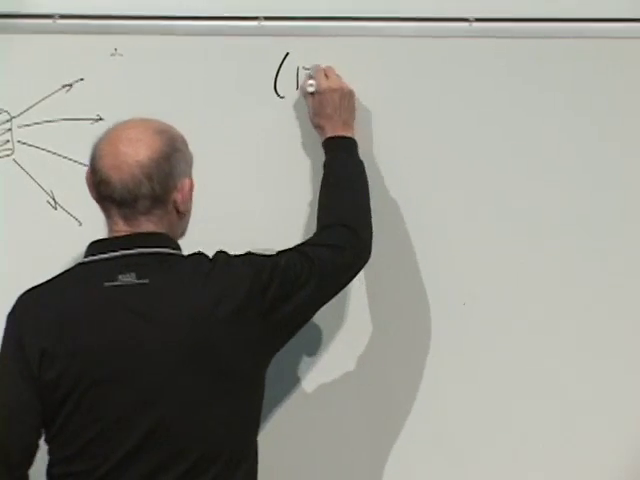
\includegraphics[width=0.66\textwidth]{lecture_06_figure_02.png}
  \caption{La condición de capa de masa en la convención métrica empleada a lo largo de la clase.}
  \lectureframe{00:05:56}
  \label{fig:l06-mass-shell}
\end{figure}

Consideremos dos partículas entrantes con momentos \(k_1,k_2\) y dos partículas salientes con momentos físicos \(q_3,q_4\). La conservación de la energía y el momento se expresa mediante una sola ecuación de cuatro vectores:
\begin{equation}
  k_1+k_2=q_3+q_4.
  \label{eq:l06-physical-conservation}
\end{equation}
Es conveniente asignar un momento entrante a cada línea externa:
\begin{equation}
  k_3\equiv-q_3,
  \qquad
  k_4\equiv-q_4.
\end{equation}
Entonces,
\begin{equation}
  k_1+k_2+k_3+k_4=0,
  \label{eq:l06-all-incoming}
\end{equation}
y cada pata satisface \(k_i^2=-m_i^2\). En esta convención contable, las partículas salientes tienen energía negativa; sus energías físicas siguen siendo positivas.

\begin{figure}[H]
  \centering
  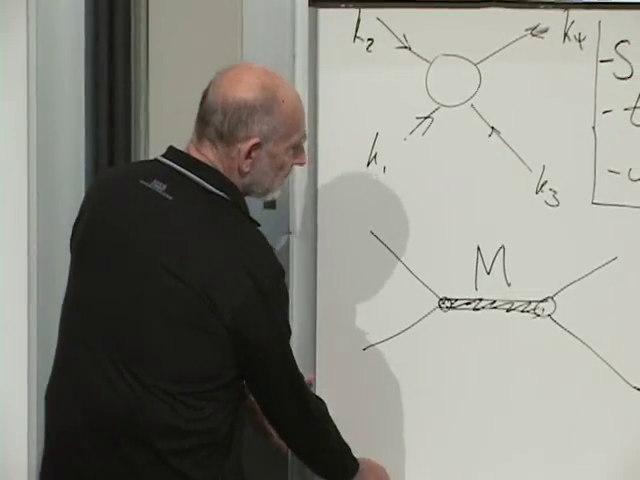
\includegraphics[width=0.68\textwidth]{lecture_06_figure_03.png}
  \caption{Se invierten los momentos físicos salientes para poder tratar simétricamente como entrantes los cuatro momentos externos.}
  \lectureframe{00:09:10}
  \label{fig:l06-all-incoming-board}
\end{figure}

Al principio, la amplitud parece ser una función de dieciséis componentes, \(\mathcal A(k_1,k_2,k_3,k_4)\). La mayoría son redundantes. Pasemos al sistema del centro de masas, orientemos los momentos entrantes a lo largo de un eje elegido y supongamos, para simplificar, que las cuatro partículas tienen la misma masa. El estado entrante queda entonces determinado por un solo número: la energía del centro de masas. Los momentos espaciales salientes deben ser iguales y opuestos, y tener el mismo módulo que los del par entrante. Solo queda el ángulo de desviación \(\theta\). Por tanto, el proceso tiene dos variables cinemáticas independientes:
\begin{equation}
  E_{\mathrm{cm}},
  \qquad
  \theta.
  \label{eq:l06-two-data}
\end{equation}

\section{Variables de Mandelstam}

Las dos cantidades físicas de \eqref{eq:l06-two-data} deberían poder expresarse sin elegir un sistema de referencia. Con la convención de todos entrantes, definamos
\begin{equation}
  \begin{aligned}
    -s&=(k_1+k_2)^2,\\
    -t&=(k_1+k_3)^2,\\
    -u&=(k_1+k_4)^2.
  \end{aligned}
  \label{eq:l06-mandelstam}
\end{equation}
En el sistema del centro de masas, las partes espaciales de \(k_1+k_2\) se cancelan; por tanto,
\begin{equation}
  s=E_{\mathrm{cm}}^2.
  \label{eq:l06-s-energy}
\end{equation}

Para un momento físico saliente \(q_3=-k_3\),
\begin{equation}
  k_1+k_3=k_1-q_3
\end{equation}
es el momento transferido de la pata 1 a la pata 3. Para masas externas iguales y un módulo del momento espacial entrante de \(p\),
\begin{equation}
  -t=2p^2(1-\cos\theta),
  \qquad
  -u=2p^2(1+\cos\theta).
  \label{eq:l06-tu-angle}
\end{equation}
Así, \(t\) y \(u\) contienen la información angular que miden los detectores.

\begin{figure}[H]
  \centering
  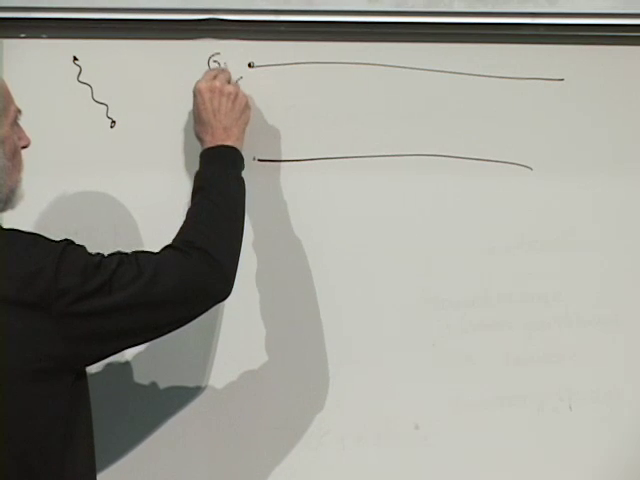
\includegraphics[width=0.74\textwidth]{lecture_06_figure_04.png}
  \caption{Las definiciones simétricas de \(s,t,u\) con la convención de todos entrantes.}
  \lectureframe{00:26:20}
  \label{fig:l06-stu-board}
\end{figure}

Que haya tres símbolos no significa que existan tres datos independientes. Al elevar al cuadrado \eqref{eq:l06-all-incoming} y usar \(k_i^2=-m^2\), se obtiene
\begin{equation}
  s+t+u=4m^2
  \label{eq:l06-stu-constraint}
\end{equation}
para masas iguales. Una vez conocidos \(s\) y \(t\), \(u\) queda determinado.

\begin{classroomqa}\audiencequestion{¿Podría el vacío frenar una partícula en movimiento libre, como si hubiera fricción? \lecturetimestamp{00:27:17}}\lecturerresponse{No en un vacío invariante bajo traslaciones. No hay dónde transferir el momento que falta, así que la conservación del momento prohíbe esa fricción. Se puede imaginar un medio u otro vacío que seleccione un sistema de reposo privilegiado, pero ese no es el vacío que consideramos aquí.}\end{classroomqa}

\begin{classroomqa}\audiencequestion{¿Por qué las dos partículas salientes deben tener la misma energía? \lecturetimestamp{00:27:54}}\lecturerresponse{En el sistema del centro de masas, sus momentos espaciales deben ser iguales y opuestos. En el proceso de masas iguales que estamos considerando, módulos de momento iguales implican energías iguales mediante \(E^2=p^2+m^2\). Si las masas de las partículas salientes fueran distintas, habría que modificar esa última conclusión.}\end{classroomqa}

\section{Canales directo y cruzado}

Un sencillo diagrama de partículas puntuales permite que las partículas 1 y 2 formen una partícula intermedia de masa \(M\), que luego se desintegra en 3 y 4. Salvo por factores en el numerador y la prescripción del polo, la dependencia característica es
\begin{equation}
  \mathcal A_s\sim\frac{g^2}{s-M^2}.
  \label{eq:l06-s-channel}
\end{equation}
Este es el proceso del canal directo, o canal \(s\). Si se gira la conectividad, se obtiene el intercambio entre las dos líneas externas:
\begin{equation}
  \mathcal A_t\sim\frac{g^2}{t-M^2},
  \label{eq:l06-t-channel}
\end{equation}
el proceso del canal cruzado, o canal \(t\). Una tercera conectividad da
\begin{equation}
  \mathcal A_u\sim\frac{g^2}{u-M^2}.
  \label{eq:l06-u-channel}
\end{equation}

\begin{figure}[H]
  \centering
  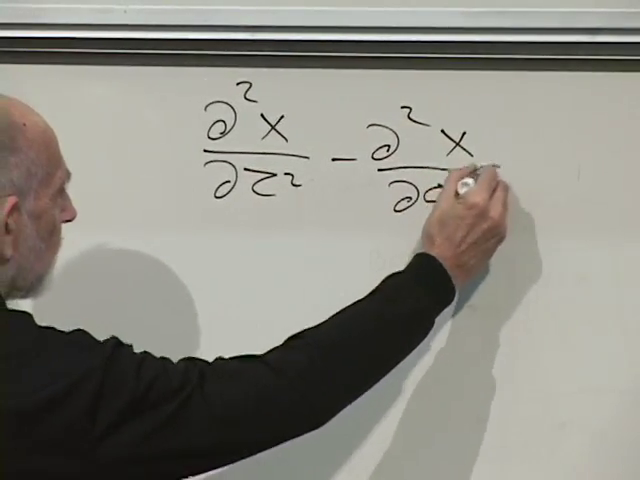
\includegraphics[width=0.72\textwidth]{lecture_06_figure_05.png}
  \caption{Producción directa mediante un estado intermedio y el polo correspondiente \(g^2/(s-M^2)\); la conectividad cruzada se está montando en el mismo tablero.}
  \lectureframe{00:30:50}
  \label{fig:l06-channel-board}
\end{figure}

La distinción es física. A este nivel escalar rudimentario, \eqref{eq:l06-s-channel} depende de la energía de colisión, pero no del ángulo. El estado compuesto ha perdido la dirección incidente antes de desintegrarse, por lo que su desintegración es isótropa. La amplitud de intercambio depende de la transferencia de momento y, por tanto, del ángulo; una partícula intercambiada ligera favorece mucho las desviaciones pequeñas. El espín añadiría más dependencia angular, pero la estructura de polos ya es visible.

\begin{classroomqa}\audiencequestion{¿El canal \(u\) que falta da lugar a un tercer término? \lecturetimestamp{00:34:47}}\lecturerresponse{Sí, siempre que las identidades de las partículas y sus acoplamientos permitan esa conectividad. En ese caso se incluye un término con un polo en \(u=M^2\). No es una nueva variable cinemática independiente, porque \(s+t+u=4m^2\), pero sí corresponde a un diagrama de canal distinto.}\end{classroomqa}

\section{Una función, dos descripciones de canal}

Un solo polo es un modelo pobre para la dispersión de mesones. Dos mesones pueden formar muchas resonancias, con una torre de masas y momentos angulares. La primera respuesta en la década de 1960 fue añadir más polos del canal \(s\), más polos del canal \(t\) y los polos permitidos del canal \(u\). Entonces se encontró una función mucho más económica. En las unidades de la clase, donde la trayectoria de Regge lineal y su intercepto se han absorbido en \(s\) y \(t\), la función es
\begin{equation}
  \mathcal A_{\mathrm V}(s,t)
  \propto
  \frac{\Gamma(-s)\Gamma(-t)}{\Gamma(-s-t)}.
  \label{eq:l06-veneziano}
\end{equation}
La función gamma extiende el factorial:
\begin{equation}
  \Gamma(n)=(n-1)!
\end{equation}
para enteros positivos.

\begin{figure}[H]
  \centering
  \includegraphics[width=0.68\textwidth]{lecture_06_figure_06.png}
  \caption{La amplitud de Veneziano escrita como un cociente simétrico de funciones gamma.}
  \lectureframe{00:42:25}
  \label{fig:l06-veneziano-board}
\end{figure}

Los polos de \(\Gamma(-s)\) reproducen una torre infinita de resonancias del canal directo. Sin embargo, la misma expresión es simétrica bajo \(s\leftrightarrow
t\), así que sus polos \(\Gamma(-t)\) dan una expansión del canal cruzado. No se trata de dos contribuciones añadidas por separado. Una sola función analítica admite ambas descripciones. Esta es la antigua idea de la dualidad entre las resonancias del canal directo y los intercambios del canal cruzado.

\begin{classroomqa}\audiencequestion{¿Cómo puede una amplitud contener las sumas de ambos canales sin sumarlas entre sí? \lecturetimestamp{00:43:32}}\lecturerresponse{Esa es precisamente la sorpresa. Al desarrollar la función cerca de sus polos del canal \(s\), se organiza como una serie de resonancias directas; al desarrollarla cerca de sus polos del canal \(t\), la misma función se organiza como una serie de intercambios. Hace falta un modelo microscópico que explique por qué ambas interpretaciones son la misma, y ese modelo es una cuerda interactuante.}\end{classroomqa}

\section{Una banda barrida por una cuerda abierta}

Parametricemos una cuerda abierta mediante
\begin{equation}
  0\leq\sigma\leq\pi.
\end{equation}
La etiqueta \(\sigma\) no es una posición en el espacio-tiempo. La inmersión \(X^\mu(\sigma,\tau)\) indica dónde se encuentra en el espacio-tiempo el punto que lleva esa etiqueta, mientras que \(\tau\) mide la evolución. Una partícula puntual barre una línea de mundo; una cuerda en movimiento barre una hoja de mundo bidimensional. En la teoría libre, cada coordenada de inmersión satisface
\begin{equation}
  \frac{\partial^2X^\mu}{\partial\tau^2}
  -
  \frac{\partial^2X^\mu}{\partial\sigma^2}
  =0.
  \label{eq:l06-wave-equation}
\end{equation}

\begin{figure}[H]
  \centering
  \includegraphics[width=0.70\textwidth]{lecture_06_figure_07.png}
  \caption{La ecuación de ondas que rige cada coordenada de la cuerda libre en la banda de la hoja de mundo.}
  \lectureframe{00:49:10}
  \label{fig:l06-wave-equation-board}
\end{figure}

Para construir la dispersión, conviene no tomar demasiado pronto el límite continuo. Sustituyamos cada cuerda por \(n\) masas puntuales unidas por resortes. La hoja de mundo se convierte en un conjunto denso de líneas de mundo próximas, y sus modos normales son osciladores armónicos ordinarios. Dos cadenas entrantes pueden tocarse por sus extremos. En ese instante se une un resorte nuevo, las cadenas evolucionan durante un tiempo \(\tau\) como una sola cadena más larga y, más adelante, se rompe un resorte para que emerjan dos cadenas salientes.

\begin{figure}[H]
  \centering
  \includegraphics[width=0.72\textwidth]{lecture_06_figure_08.png}
  \medskip

  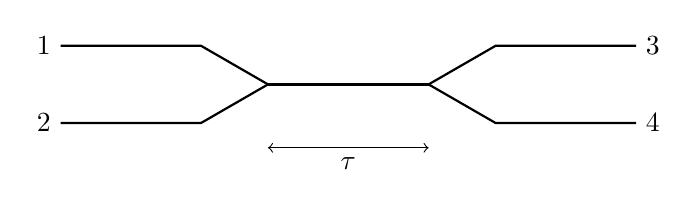
\begin{tikzpicture}[x=0.85cm,y=0.70cm]
    \draw[thick] (0,2.2) -- (2.1,2.2) -- (3.1,1.5);
    \draw[thick] (0,0.8) -- (2.1,0.8) -- (3.1,1.5);
    \draw[thick] (3.1,1.5) -- (5.5,1.5);
    \draw[thick] (5.5,1.5) -- (6.5,2.2) -- (8.6,2.2);
    \draw[thick] (5.5,1.5) -- (6.5,0.8) -- (8.6,0.8);
    \draw[<->] (3.1,0.35) -- node[below] {\(\tau\)} (5.5,0.35);
    \node[left] at (0,2.2) {1};
    \node[left] at (0,0.8) {2};
    \node[right] at (8.6,2.2) {3};
    \node[right] at (8.6,0.8) {4};
  \end{tikzpicture}
  \caption{Dos cuerdas abiertas discretizadas se tocan, forman una sola cuerda intermedia durante un tiempo \(\tau\) y se separan. El fotograma de la fuente conserva la construcción con resortes y líneas de mundo; el esquema aísla la conectividad.}
  \lectureframe{00:51:25}
  \label{fig:l06-string-joining}
\end{figure}

Las dos cuerdas solo se dibujan juntas en el espacio de parámetros. No es necesario que sus posiciones en el espacio-tiempo estén próximas hasta que las coordenadas de sus extremos coincidan efectivamente. La libertad de reparametrización permite situar los eventos de unión y separación en posiciones convenientes del diagrama; en la próxima clase, esta libertad geométrica se convertirá en simetría conforme.

\section{El cálculo de osciladores paso a paso}

Sea la primera cadena la que tiene coordenadas \(x_1,\ldots,x_n\), y la segunda, la que tiene coordenadas \(x_{n+1},\ldots,x_{2n}\). Sus coordenadas del centro de masas son
\begin{equation}
  X_{\mathrm{cm}}^{(1)}
  =\frac1n\sum_{a=1}^{n}x_a,
  \qquad
  X_{\mathrm{cm}}^{(2)}
  =\frac1n\sum_{a=n+1}^{2n}x_a.
  \label{eq:l06-chain-centers}
\end{equation}
Una cadena con momento definido \(k_1\) tiene una onda plana para el centro de masas multiplicada por el estado fundamental de los osciladores internos:
\begin{align}
  \Psi_1
  &=
  e^{ik_1\cdot X_{\mathrm{cm}}^{(1)}}
  \psi_0(x_1,\ldots,x_n),
  \\
  \Psi_2
  &=
  e^{ik_2\cdot X_{\mathrm{cm}}^{(2)}}
  \psi_0(x_{n+1},\ldots,x_{2n}).
  \label{eq:l06-two-wavefunctions}
\end{align}
Los factores \(\psi_0\) dependen de las coordenadas relativas, no de la traslación conjunta de toda la cadena. Como las cuerdas entrantes son inicialmente sistemas cuánticos separados,
\begin{equation}
  \Psi_{\mathrm{in}}=\Psi_1\Psi_2.
  \label{eq:l06-product-state}
\end{equation}

\begin{figure}[H]
  \centering
  \includegraphics[width=0.76\textwidth]{lecture_06_figure_09.png}
  \caption{Las dos ondas planas de momento y sus factores de estado fundamental de los osciladores internos, representados en colores distintos.}
  \lectureframe{00:58:05}
  \label{fig:l06-wavefunctions-board}
\end{figure}

La unión selecciona la parte de esta función de onda en la que coinciden las coordenadas de los dos extremos:
\begin{equation}
  x_n=x_{n+1}.
  \label{eq:l06-endpoint-contact}
\end{equation}
En ese instante, las demás coordenadas no cambian. A continuación, el estado evoluciona con el hamiltoniano \(H_{\mathrm{joined}}\) de la única cadena más larga:
\begin{equation}
  \Psi(\tau)
  =
  e^{-iH_{\mathrm{joined}}\tau}\Psi(0).
  \label{eq:l06-time-evolution}
\end{equation}
Por último, se calcula su solapamiento con un producto de estados de cuerdas salientes con momentos \(q_3,q_4\).

\begin{figure}[H]
  \centering
  \includegraphics[width=0.76\textwidth]{lecture_06_figure_10.png}
  \caption{La función de onda de las dos cadenas justo antes de imponer la coincidencia de los extremos.}
  \lectureframe{00:58:55}
  \label{fig:l06-endpoint-board}
\end{figure}

El cálculo es largo, pero no encierra ningún misterio. Cada coordenada interna se puede descomponer en modos de oscilación, de modo que el solapamiento en la unión, la evolución temporal y la proyección final se reducen al álgebra gaussiana de osciladores. Lo que sigue sin determinarse es el tiempo de vida \(\tau\) de la cuerda unida.

\begin{classroomqa}\audiencequestion{¿Se suman o se multiplican las funciones de onda negra y roja? \lecturetimestamp{01:02:26}}\lecturerresponse{Se multiplican. En la representación de coordenadas, el estado producto tensorial de dos sistemas independientes viene dado por el producto de sus funciones de onda. La suma describiría una superposición de alternativas, no la presencia simultánea de las dos cuerdas entrantes.}\end{classroomqa}

\begin{classroomqa}\audiencequestion{¿Por qué se integra sobre el tiempo intermedio \(\tau\)? \lecturetimestamp{01:04:04}}\lecturerresponse{No se asigna un tiempo de vida fijo a la cuerda unida. La regla de Feynman consiste en sumar las amplitudes de todas las historias posibles. En esta descripción, el parámetro continuo de historia que queda es el tiempo transcurrido entre la unión y la separación, así que la suma se convierte en una integral sobre \(0\leq\tau<\infty\).}\end{classroomqa}

\section{Del tiempo de propagación a la función beta}

Tras evaluar los solapamientos de los osciladores, el resultado puede escribirse como
\begin{equation}
  \mathcal A(s,t)
  \propto
  \int_0^\infty d\tau\,
  e^{\tau(s+1)}
  \bigl(1-e^{-\tau}\bigr)^{-t-1}
  e^{-\tau}.
  \label{eq:l06-tau-integral}
\end{equation}
Se mantiene explícito el factor final \(e^{-\tau}\) porque es el jacobiano necesario en el siguiente paso. De manera equivalente, las exponenciales primera y última se combinan para dar \(e^{s\tau}\).

\begin{figure}[H]
  \centering
  \includegraphics[width=0.76\textwidth]{lecture_06_figure_11.png}
  \caption{El integrando respecto al tiempo de propagación tras el cálculo de los osciladores; el factor \(e^{-\tau}\) separado proporciona el jacobiano del cambio de variable.}
  \lectureframe{01:06:45}
  \label{fig:l06-tau-integral-board}
\end{figure}

Hagamos ahora el cambio
\begin{equation}
  z=e^{-\tau},
  \qquad
  dz=-e^{-\tau}\,d\tau.
  \label{eq:l06-z-substitution}
\end{equation}
Cuando \(\tau\) varía de \(0\) a \(\infty\), \(z\) varía de \(1\) a \(0\). El signo menos invierte los límites y se obtiene
\begin{equation}
  \mathcal A(s,t)
  \propto
  \int_0^1
  z^{-s-1}(1-z)^{-t-1}\,dz.
  \label{eq:l06-beta-integral}
\end{equation}

\begin{figure}[H]
  \centering
  \includegraphics[width=0.74\textwidth]{lecture_06_figure_12.png}
  \caption{El cambio de variable \(z=e^{-\tau}\) hace aparecer la integral beta de Euler.}
  \lectureframe{01:08:49}
  \label{fig:l06-beta-integral-board}
\end{figure}

Esta integral se define directamente en la región donde converge en sus extremos y, fuera de ella, mediante continuación analítica. Es la función beta de Euler:
\begin{equation}
  B(-s,-t)
  =
  \frac{\Gamma(-s)\Gamma(-t)}{\Gamma(-s-t)}.
  \label{eq:l06-beta-gamma}
\end{equation}

\begin{figure}[H]
  \centering
  \includegraphics[width=0.72\textwidth]{lecture_06_figure_13.png}
  \caption{El tablero identifica la integral transformada con \(B(-s,-t)\) y empieza a recuperar su expresión en términos de funciones gamma.}
  \lectureframe{01:12:24}
  \label{fig:l06-beta-gamma-board}
\end{figure}

La simetría entre canales resulta ahora inmediata. Bajo \(z\mapsto1-z\),
\begin{equation}
  \int_0^1 z^{-s-1}(1-z)^{-t-1}\,dz
  =
  \int_0^1 z^{-t-1}(1-z)^{-s-1}\,dz.
\end{equation}
Por tanto, \(\mathcal A(s,t)=\mathcal A(t,s)\). Un proceso construido a partir de dos cuerdas que se unen y luego se separan contiene automáticamente también la descripción cruzada.
\editorialnote{En los argumentos de la función beta, la clase omite la pendiente y el intercepto de Regge. En notación estándar, se sustituye \(s,t\) por las trayectorias lineales correspondientes \(\alpha(s),\alpha(t)\). La dualidad y el argumento basado en el cambio de variable no cambian.}

\begin{classroomqa}\audiencequestion{El cociente de funciones gamma se parece a expresiones con factoriales de combinatoria. ¿Tiene una interpretación directa como conteo físico? \lecturetimestamp{01:13:22}}\lecturerresponse{Para argumentos enteros, la función beta está relacionada con un cociente como \(n!\,m!/(n+m)!\), pero aquí no se propone ningún mecanismo combinatorio. La misma función especial aparece en la integral sobre la hoja de mundo; esta semejanza no fue el camino por el que se encontró la amplitud.}\end{classroomqa}

La razón, todavía oculta, por la que una misma hoja de mundo admite ambas interpretaciones de canal es la simetría conforme. Esta permite estirar la hoja como si fuera una masa elástica sin cambiar la amplitud, convirtiendo una región de propagación larga del canal directo en una imagen de intercambio del canal cruzado. La explicación geométrica queda para la próxima clase.

\section{Qué estableció la prueba de dispersión}
\enlargethispage{3\baselineskip}
\begingroup
\setlength{\medskipamount}{3pt plus 1pt minus 1pt}

La imagen discreta de la unión dio pie a un último grupo de preguntas.

\begin{classroomqa}\audiencequestion{Si se unen por los extremos dos cadenas de \(n\) constituyentes, ¿el resultado tiene \(2n-1\), y podría eso cambiar la paridad fermiónica? \lecturetimestamp{01:16:16}}\lecturerresponse{En la imagen hadrónica de los extremos, el par de extremos que se toca puede interpretarse como un par partícula-antipartícula que se aniquila, por lo que el número se reduce en dos, no en uno. En el límite continuo, la diferencia finita entre \(2n\) y \(2n-2\) no importa, pero conservar la paridad fermiónica sí importa. Los constituyentes de la red solo sirven como regulador de la cuerda continua; no son bolitas fundamentales literales.}\end{classroomqa}

\begin{classroomqa}\audiencequestion{¿La discusión posterior abordará toda la matemática de las supercuerdas? \lecturetimestamp{01:18:05}}\lecturerresponse{Solo se usarán algunas consecuencias. El camino inmediato pasa por la simetría de la hoja de mundo y la compactificación, y luego parte de un enfoque distinto desarrollado a mediados de la década de 1990: la teoría M. Su propósito es llegar a la misma física desde un punto de vista que vuelve transparentes varias características que, de otro modo, son complicadas.}\end{classroomqa}

\begin{classroomqa}\audiencequestion{¿Esta regla de unión era solo una pista obtenida de las colisiones de mesones? \lecturetimestamp{01:20:02}}\lecturerresponse{La dispersión de mesones proporcionó la pista histórica, pero la regla es general para las cuerdas abiertas. La misma topología describe las colisiones de fotones de cuerda abierta y de otros estados de cuerda abierta. Dos cuerdas cerradas se unen y se separan mediante una construcción análoga, con una cuerda cerrada en la región intermedia.}\end{classroomqa}

\begin{classroomqa}\audiencequestion{¿El cálculo se aplica solo cuando los estados de cuerda son fermiones? \lecturetimestamp{01:20:56}}\lecturerresponse{No. El cálculo original de Veneziano corresponde a la cuerda abierta bosónica. Las supercuerdas requieren grados de libertad fermiónicos adicionales y modifican detalles del integrando, pero la lógica de unión, propagación, proyección y dualidad de la hoja de mundo sigue siendo muy similar.}\end{classroomqa}

Encontrar un estado de espín uno o espín dos en el espectro de osciladores era sugerente, pero no concluyente. Las amplitudes de dispersión de esos estados proporcionaron una prueba más sólida. Las amplitudes de fotones satisfacen las identidades asociadas a la conservación de la carga y la invariancia gauge; las de gravitones satisfacen las restricciones correspondientes a un campo sin masa de espín dos. Los estados de cuerda superaron estas pruebas en interacciones con estados masivos y sin masa, así como entre sí. Por eso, las denominaciones de fotón y gravitón pasaron a ser identificaciones físicas, en lugar de conjeturas basadas solo en contar polarizaciones.
\editorialnote{En lenguaje moderno, estas pruebas se expresan mediante la desacoplación de las polarizaciones no físicas, las identidades de Ward gauge y el acoplamiento universal de baja energía del estado sin masa de espín dos.}

\begin{classroomqa}\audiencequestion{¿De dónde proviene la propia carga eléctrica en la descripción de cuerdas? \lecturetimestamp{01:24:03}}\lecturerresponse{La clase termina dejando abierta esa pregunta. Su respuesta requiere la estructura interna y la estructura de los extremos de la teoría de cuerdas, que todavía no se han presentado; por eso corresponde a la discusión que sigue, no a esta derivación de la dispersión.}\end{classroomqa}
\endgroup
